\begin{figure}[h!]
    \centering
    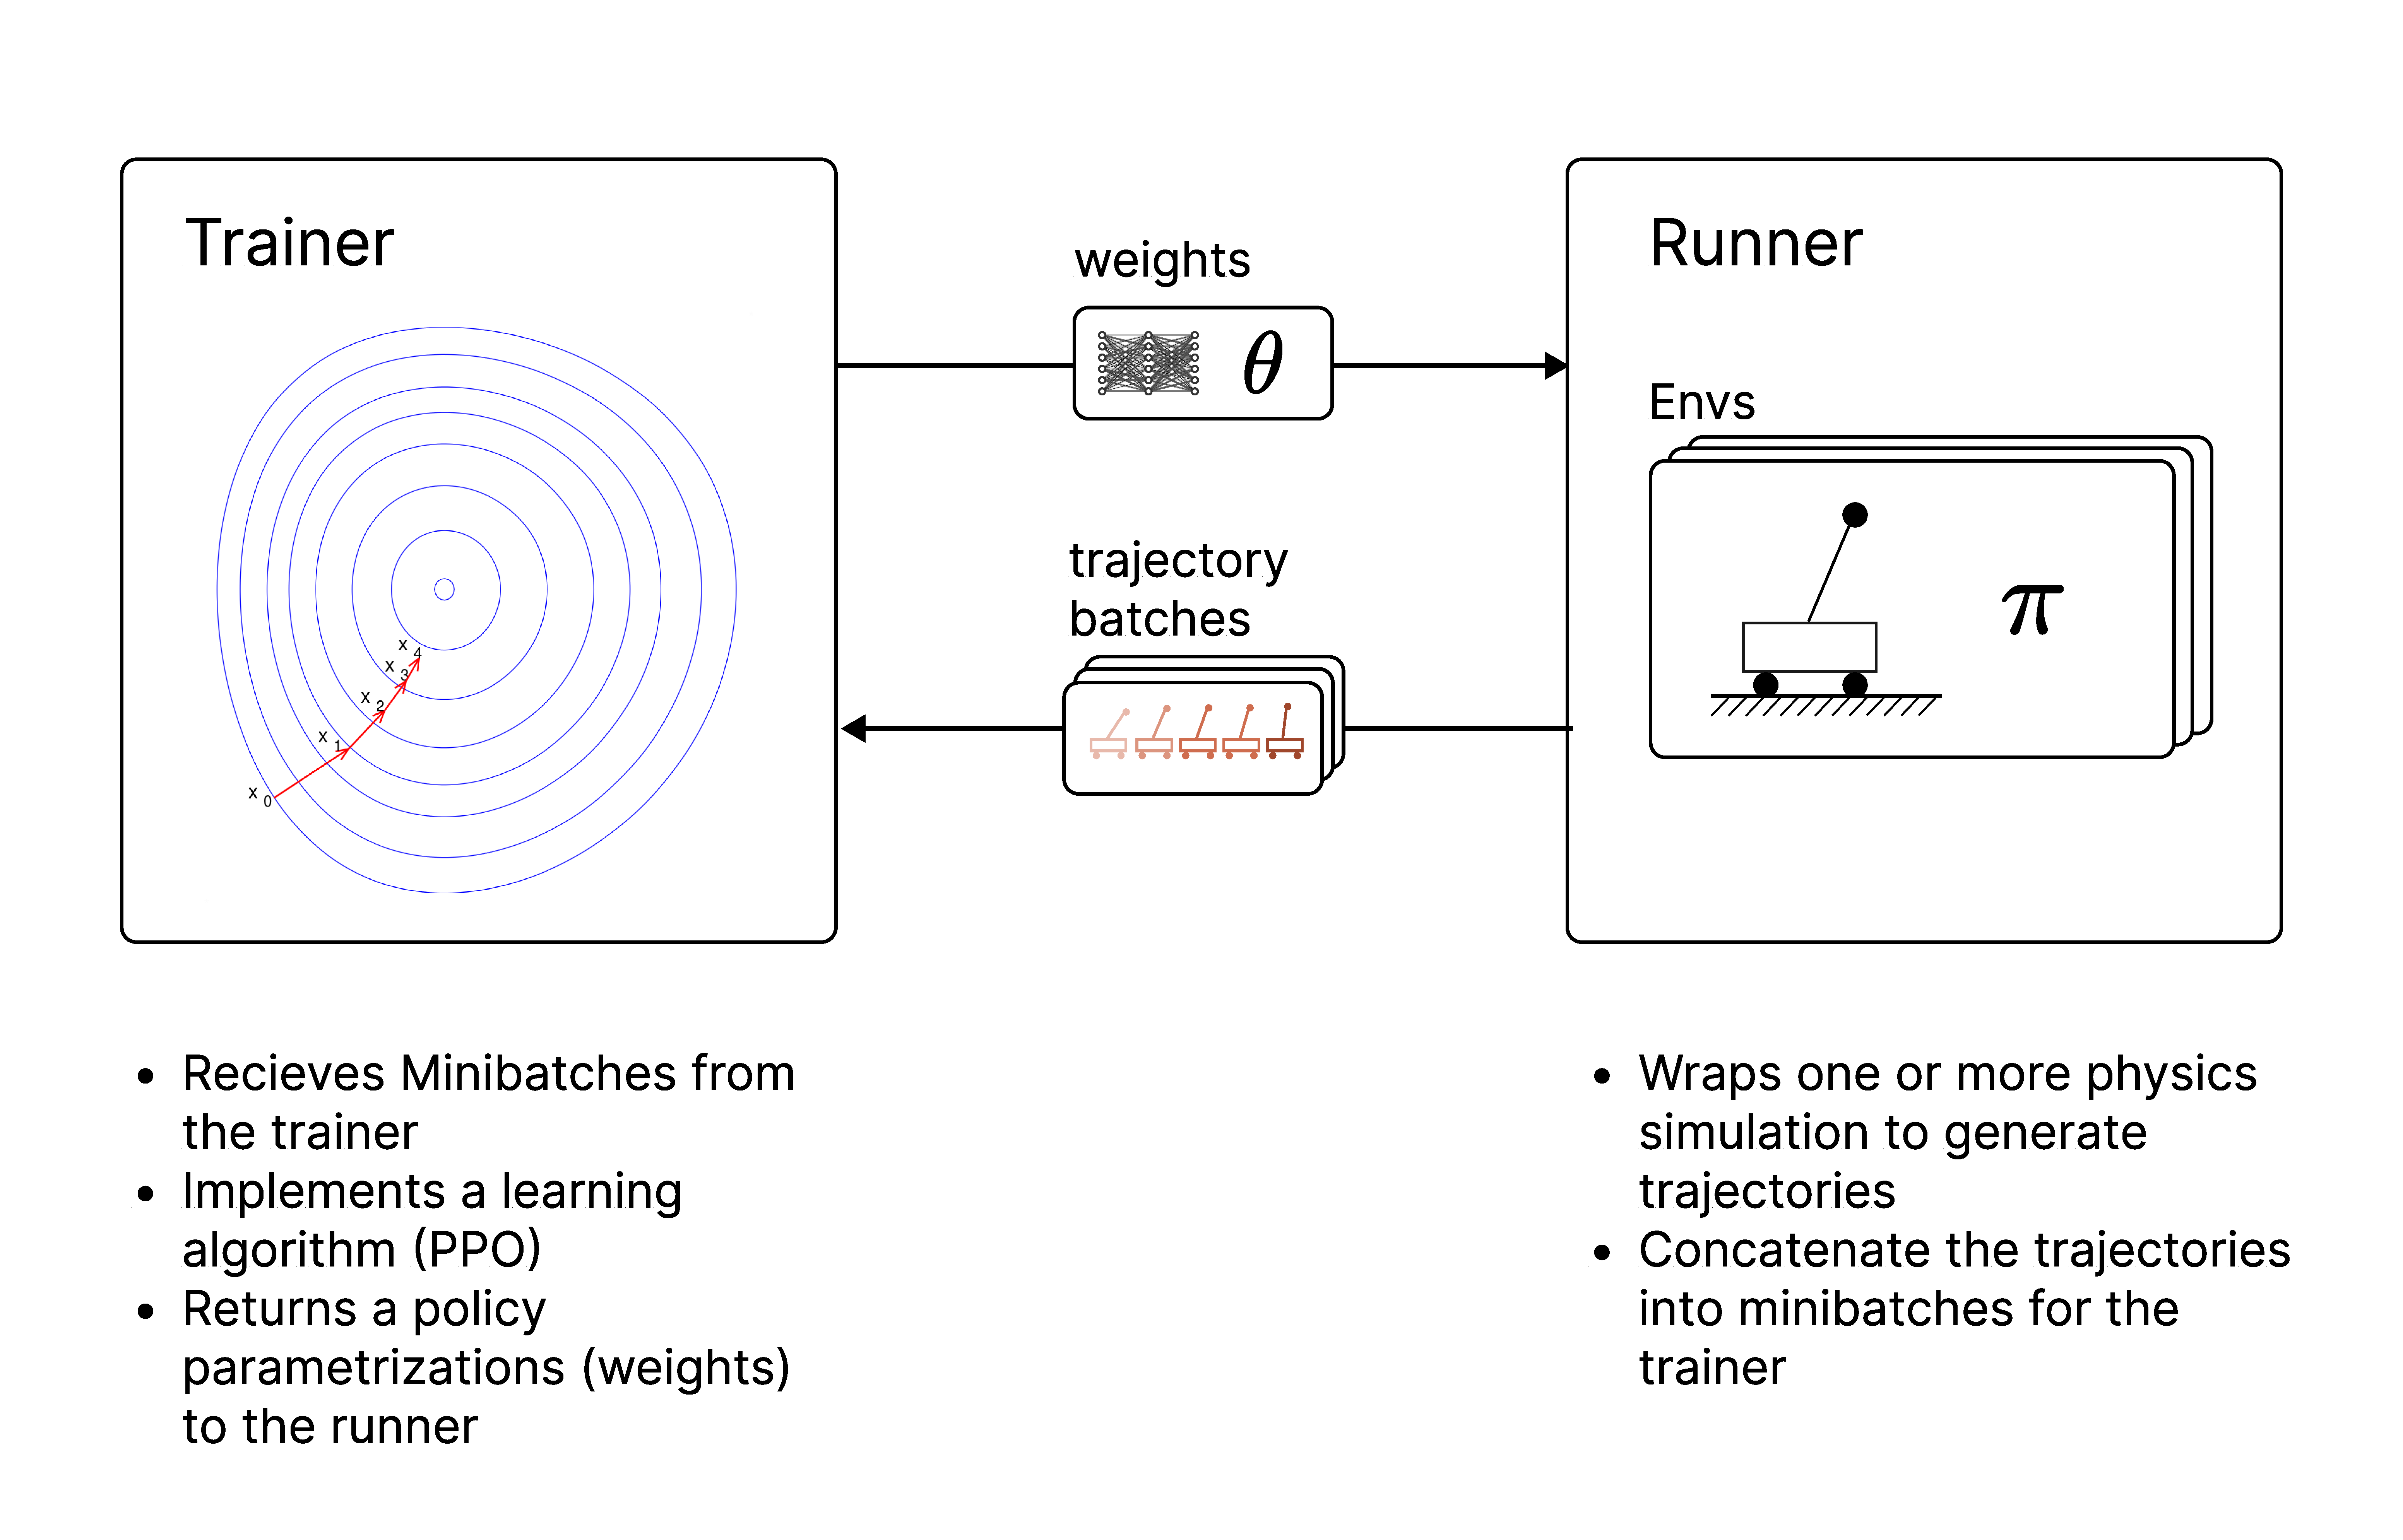
\includegraphics[width=0.45\textwidth]{figures/Framework.pdf}
    \caption{An illustration of the main components of a reinforcement learning framework. The two main components are left: an implementation of the RL algorithm, and right a wrapper for physics simulations (or environment as they are often called in the RL literature). One of the key functions of such a system is handling the trajectories generated by the environment and converting them into mini-batches, depending on the framework this can be done as part of the runner or trainer components.}
\end{figure}

The reinforcement learning-based training of a time-continuous neuron cell requires the setup of a learning environment. Such an environment must be able to:
\begin{enumerate}
    \item simulate the POMDP (since we investigate a continuous control task, this is the physics of our controlled system),
    \item implement the policy model (in our case our time-continuous neuron cells) which we discussed in section \ref{sec:nn_cell},
    \item train it using our RL algorithm (PPO) which we discussed discussed in section \ref{sec:ppo}.
\end{enumerate}

Because of the complexity of such an environment we make use of a reinforcement learning framework that structures the data collection, the learning and the evaluation of RL policies. The reinforcement learning research community has come up with several such frameworks, notable examples are \textit{stable baselines} \cite{stable-baselines}, \textit{stable baselines 3} \cite{stable-baselines3}, \textit{Ray RLLib} \cite{rllib} and \textit{ACME} \cite{hoffman2020acme}. The requirements of our project lead us to seriously consider two main frameworks: \textit{Ray RLLib} \cite{rllib} and the less known \textit{DERL} \cite{konobeev2018},  which we will now compare in further details.

\subsection{Ray RLLib}

Our first investigation into the problem we stated were performed within the \textit{Ray RLLib} framework. \textit{Ray} is an open source machine learning framework intended form large-scale distributed computing, its development started at UC Berkley's RISE Lab. \textit{Ray RLLib} \cite{rllib} is a reinforcement learning framework built on top of \textit{Ray} with the intent of allowing for fast training of RL policies on distributed hardware (for instance on a cluster). Ray features implementation of most state of the art reinforcement learning algorithms (for instance \textit{PPO}, it's asynchronous variant \textit{APPO}, \textit{IMPALA}, various Q-learning derivatives as well as imitation learning algorithms) and bindings with most environments used for continuous control (most notably \textit{PyBullet} and \textit{Mujoco}). \textit{RLLib} allows for implementing policies with either \textit{tensorflow} \cite{tensorflow2015-whitepaper} or \textit{pytorch} \cite{PytorchPaper}. \\

The main argument for the use of \textit{RLLib} is the performance it provides when deployed on a cluster, furthermore much of my direct supervisor Dr. Bellegarda's work on reinforcement learning for the control of complex quadruped robots was performed within this framework, which may open a door to experiments on such systems with less work involved. \\

Nonetheless I ended up abandoning \textit{RLLib}, this is because of several drawbacks, first most \textit{RLLib}'s implementation either do not support recurrent policies and are often shipped with bugs for recurrent policies \cite{RLLib_Bug}. This lack of support of recurrent policies makes the implementation of recurrent continuous time cells such as the ones we discuss in section \ref{sec:nn_cell}, and the fact that \textit{RLLib}'s documentation doesn't clearly specifies which model classes are unsupported further complicates the work. The second big argument for abandoning RLLib is the high complexity of implementing relatively simple changes to algorithms within the framework, this is partly a product of the fact that RLLib applications work as independent processes networked together. This makes the debugging of RLLib applications especially difficult. Furthermore the size of \textit{Ray}'s codebase further participates in slowing the process.

\subsection{DERL}

\textit{DERL} \cite{konobeev2018} is a lightweight reinforcement learning framework providing implementations of \textit{PPO}, \textit{SAC}, \textit{A2C} and \textit{DQN}.